\subsection{System level}
	The following graph is our system level state chart, which contains all our class level state charts. It shows how all classes interact.

	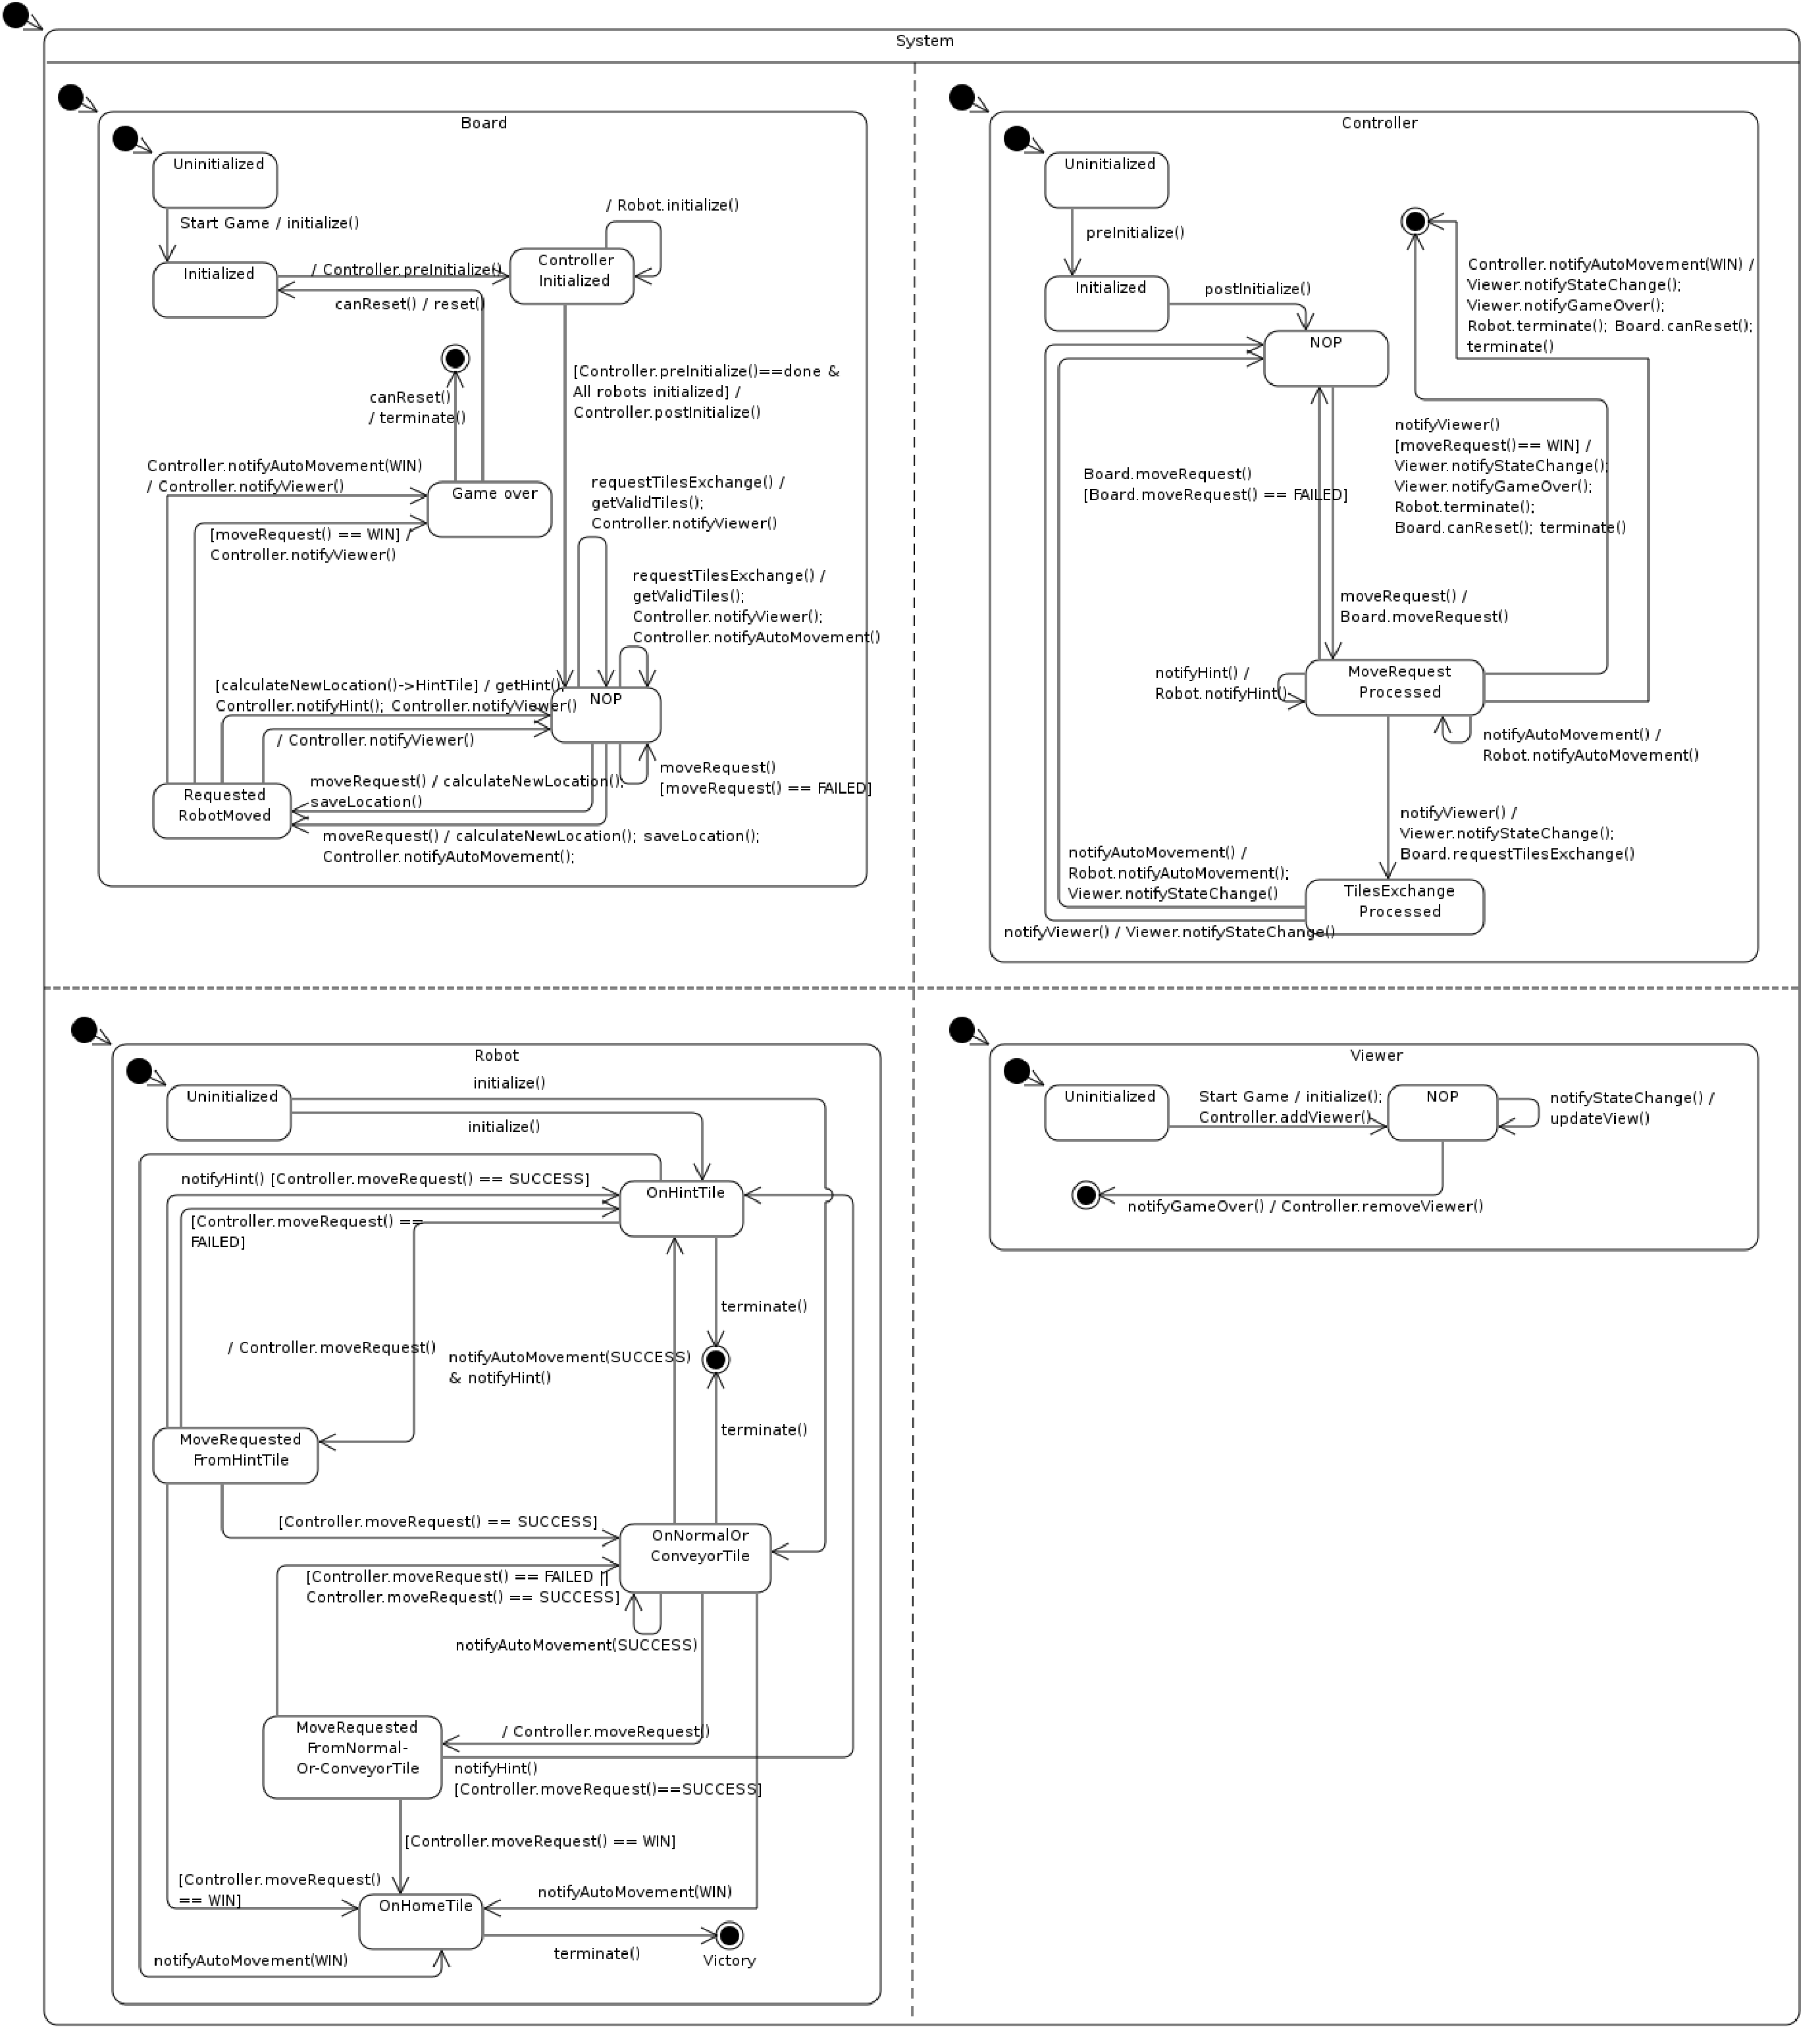
\includegraphics[width=\linewidth]{statecharts/system.pdf}

\subsection{Class level}
	\subsubsection{Board}
	First the board is initialized, then the board has to initialize the controller. After that the board goes to the NOP state from which It can answer requests from robots to move, it can also notify robots if they receive a hint, win the game or get moved by the board. After every time the board has done anything it returns to the NOP state, except when a robot has reached it's hometile, then the board has to terminate other classes via the reset() function. After the game is over the board can either terminate or go back to the initialized state to start a new game.
	
	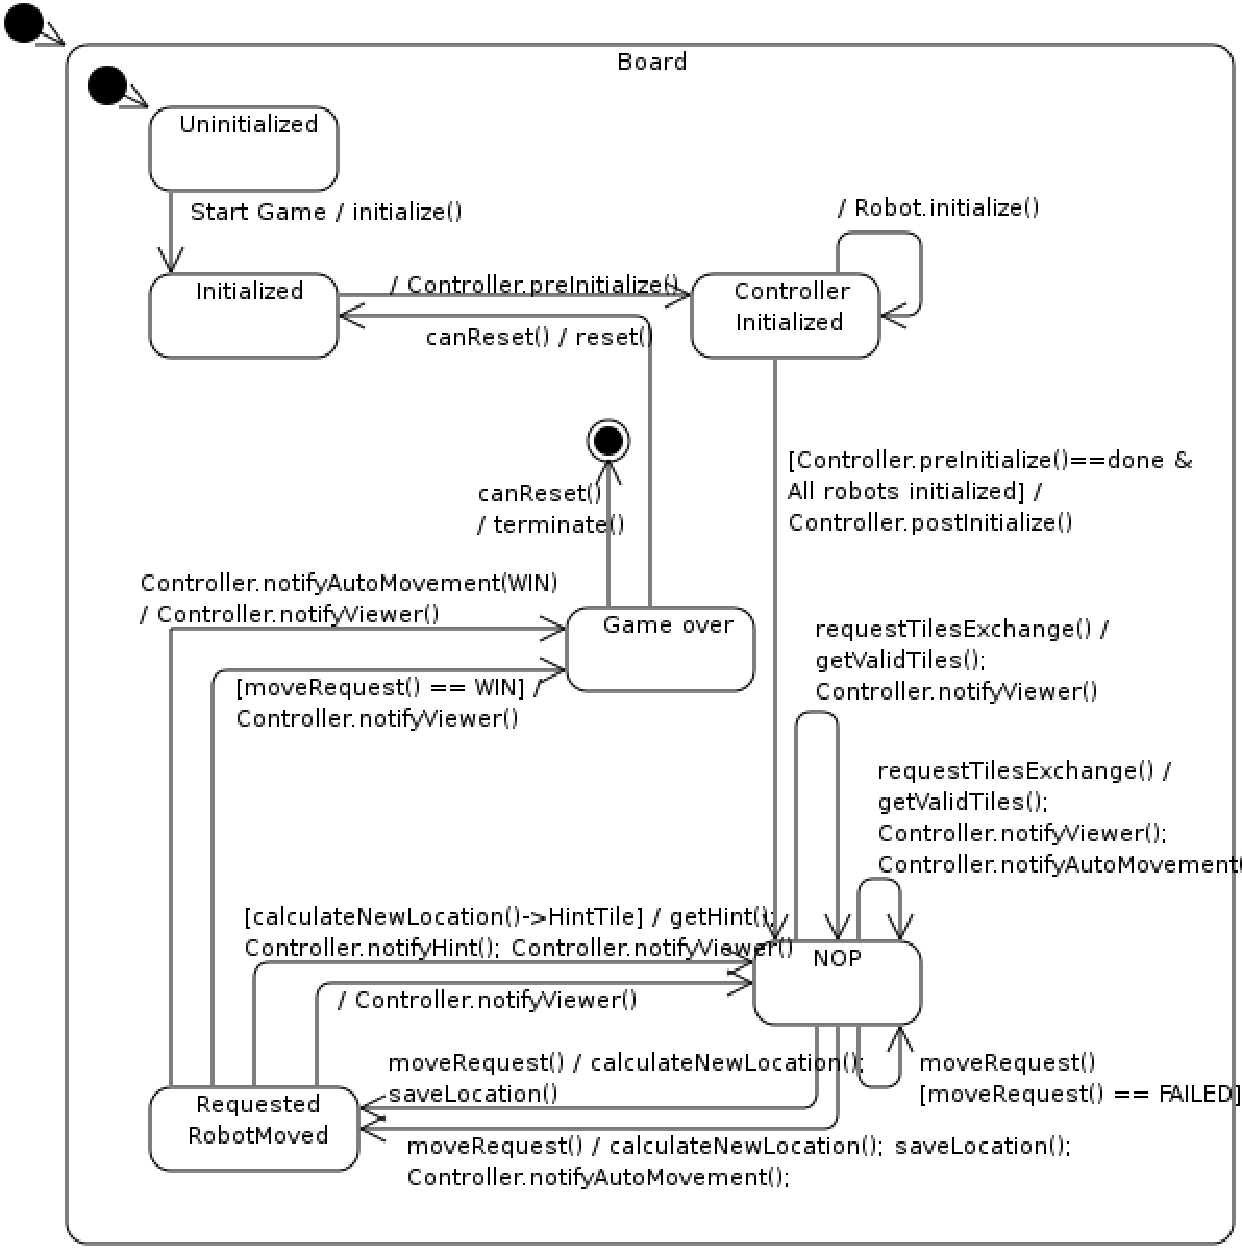
\includegraphics[width=\linewidth]{statecharts/board.pdf}

	\subsubsection{Controller}
	The controller initializes in 2 phases, the first phase is the preInitialize() function and the second phase is the postInitialize() function. After the postInitialize the class is in the NOP state from which all events take place, the controller can pass on the requestSnapshot() function from the board on to the viewer class. The controller also passes on move requests from the robot to the board, but because the  board has to answer the request the controller goes to a MoveRequestProcessed during which he waits for the board to answer. After the moverequest has been answered and it was successful 2 tiles are switched and, if needed, the moved robots receive a notifyAutoMovement(), after the tiles have been switched, the controller returns to the NOP state and it can do everything all over again. If a robot requests a move and the board class answers that the robot has reached its hometile the control will terminate because the game is over.

	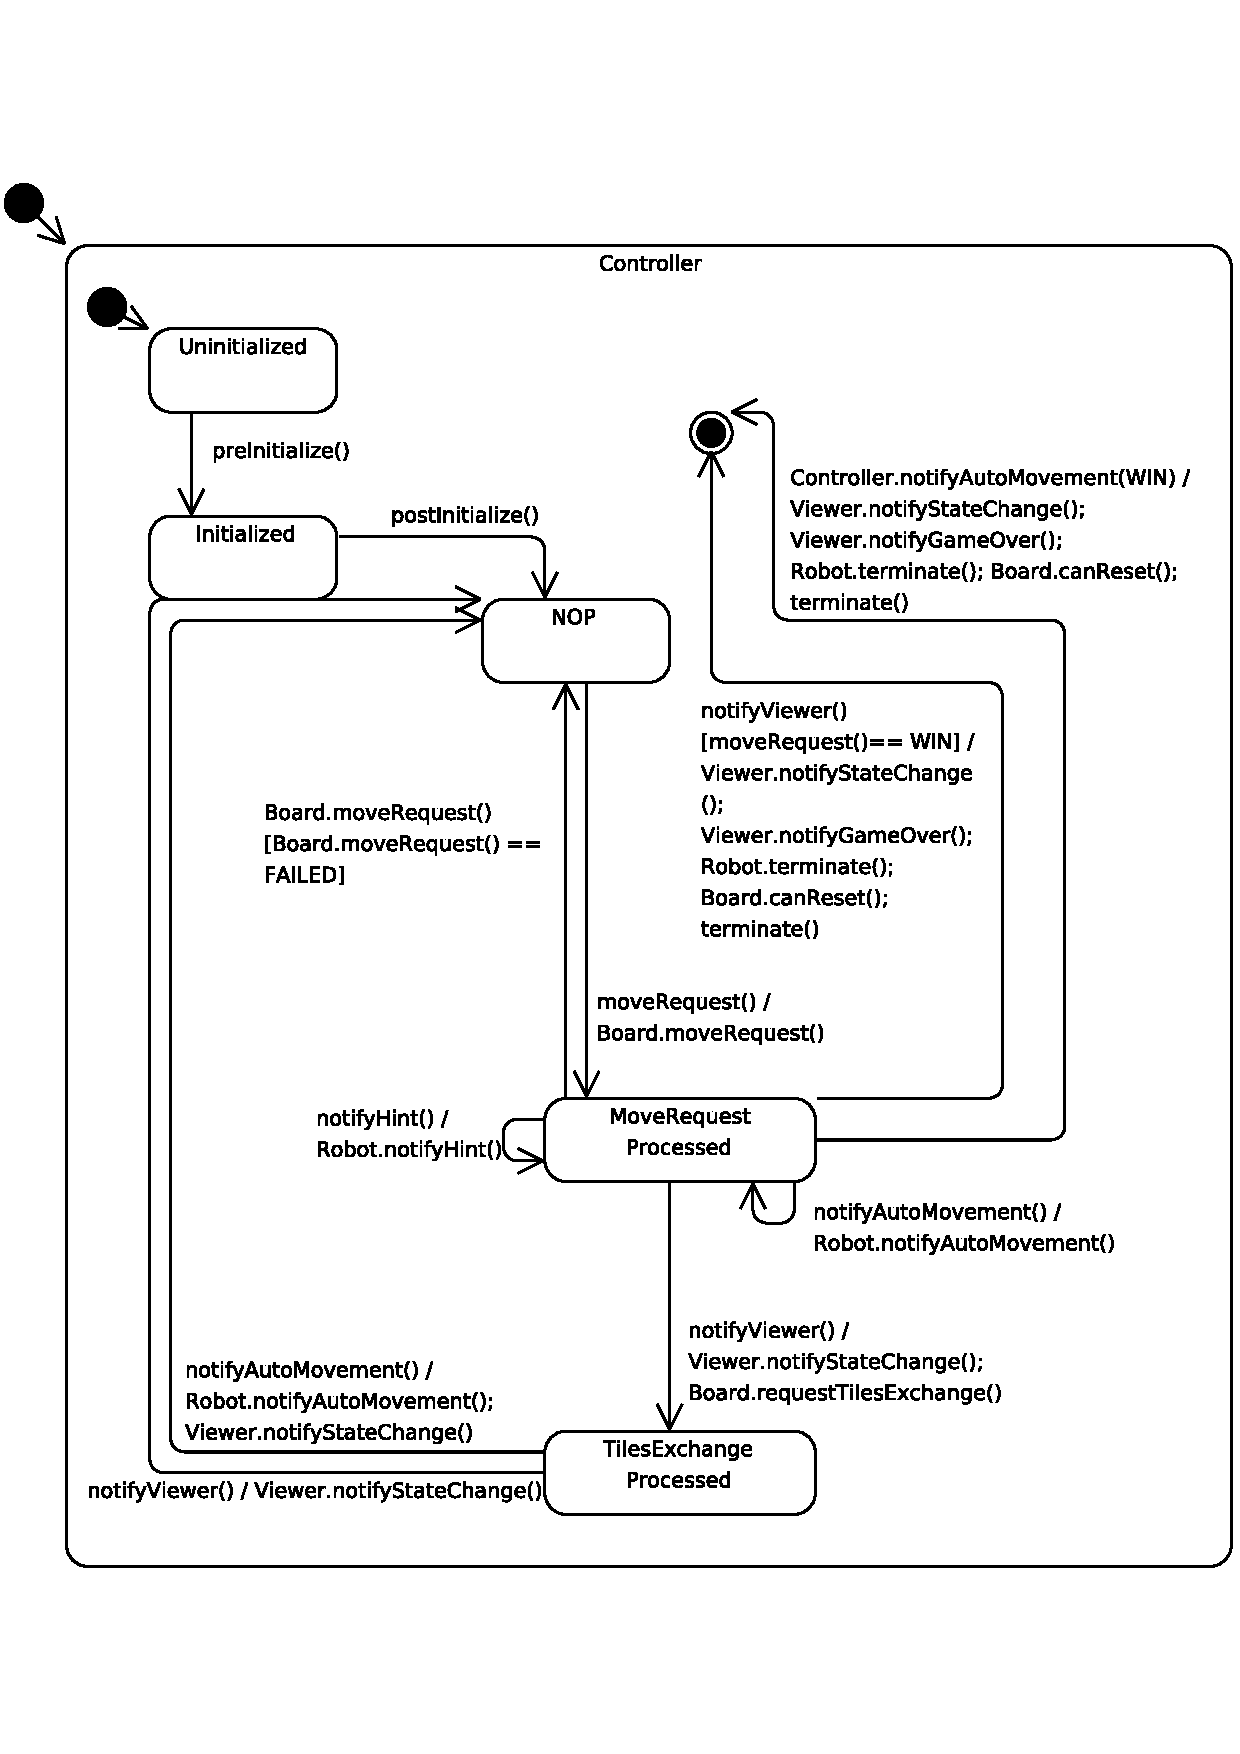
\includegraphics[width=\linewidth]{statecharts/controller.pdf}

	\subsubsection{View}
	After being initialized the viewer comes in the NOP state, which means that it isn't doing anything, but it checks the board for changes via the Controller.requestBoardStatus() function every now and then. If the board has been changed the function updateView() is called to make the changes visible, it also sends out a notifyStateChange() to let the other classes know the state has changed. The viewer is removed when the game is over, but it can also decide to remove itself.
	
	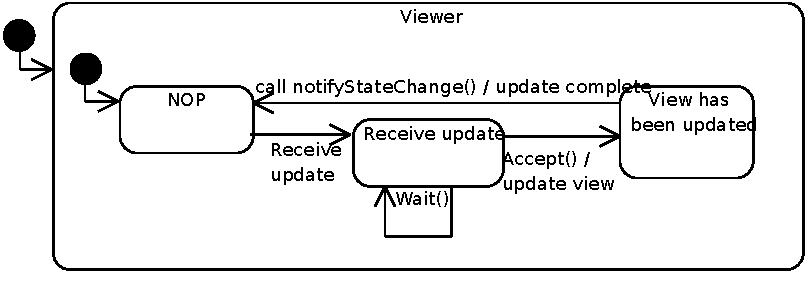
\includegraphics[width=\linewidth]{statecharts/view.pdf}

	\subsubsection{Robot}
	The robot class gets initialized by the controller, it starts at a randomly picked spot, which can be a normal tile, a hint tile or a conveyer tile. The robot receives a notifyAutomovement() every time it gets moved, this can happen in 2 ways: the robot steps on a conveyer belt or the robot gets moved via a tileswitch. Whenever a robot is on a tile It can request a move which can result in 3 ways: success, failed or win. If a move request is a success, the move is made, if a move request is a failure, the move is not made because the desired path of the moved Is blocked, if a move request results in a win it means that the robot has reached its hometile the game ends and this robot has won. When another robot wins this robot gets a terminate request from the controller and the game is over. The robot can also encounter hint tiles which point the robot to the location of its hometile.
	
	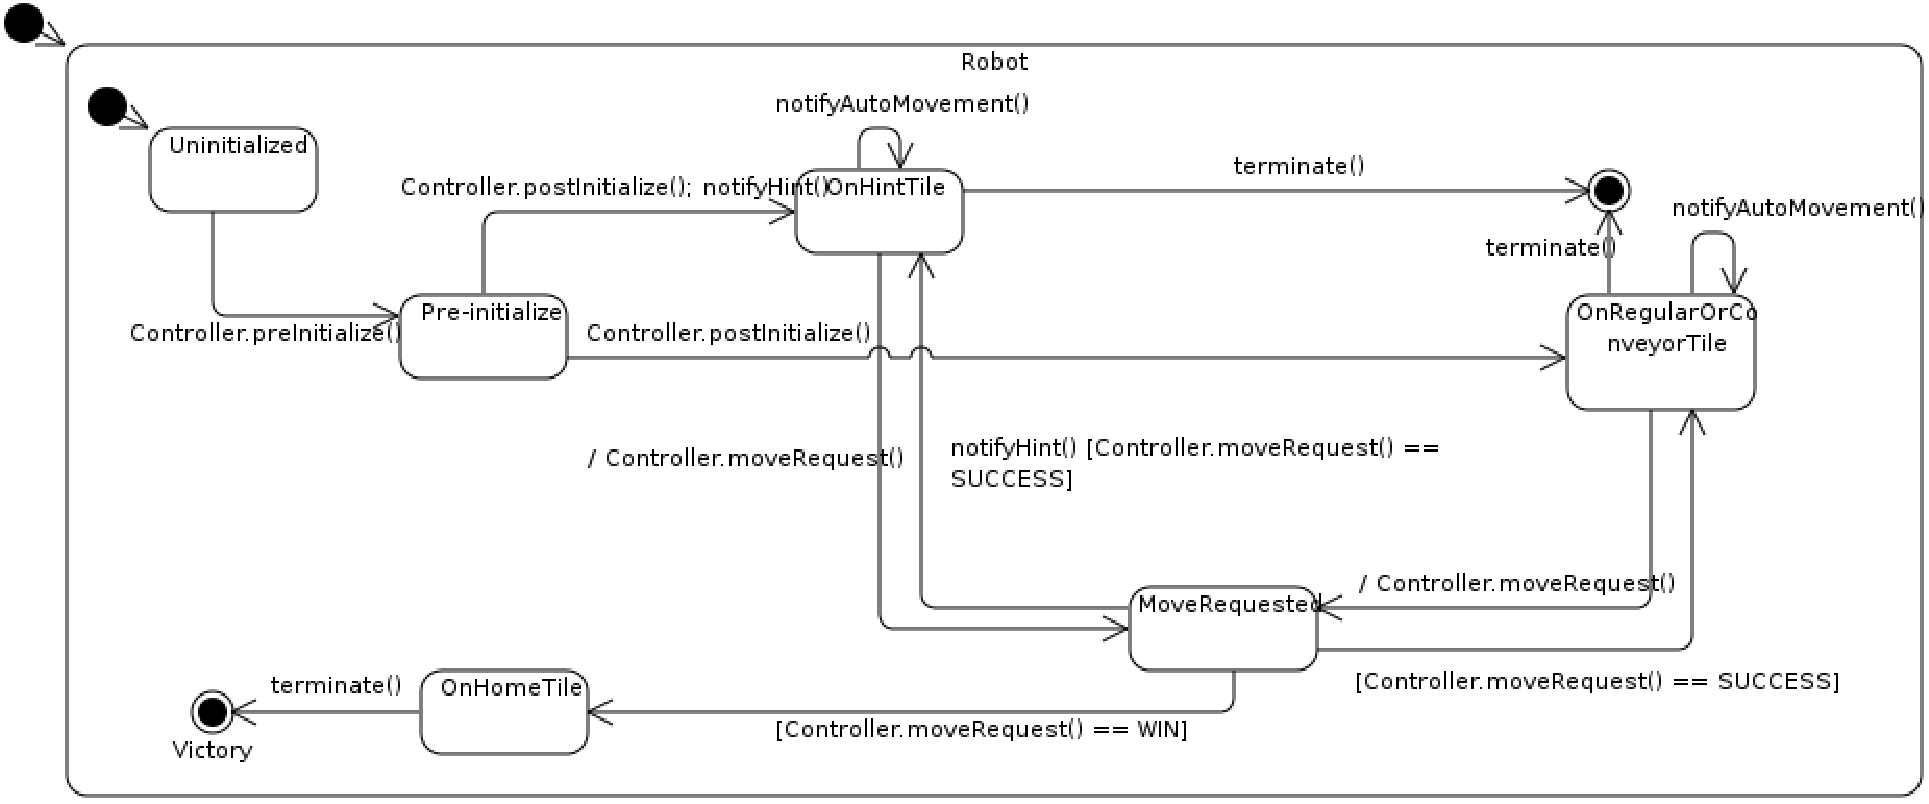
\includegraphics[width=\linewidth]{statecharts/robot.pdf}
	

	
